% Autor: Simon May
% Datum: 2014-08-19

% Zähler "fibelbeerctr" und "fibeltotalbeerscore" sind für den
% "\fibelbeertable"-Befehl
\newcounter{fibelbeerctr}
\newcounter{fibeltotalbeerscore}

% Befehl "\fibelbeerscore": Wandelt die angegebene Zahl in eine entsprechende
% Anzahl von Bildern ("Bierpunkten") um
\newcommand{\fibelbeerscore}[1]{
\addtocounter{fibeltotalbeerscore}{#1}
\forloop{fibelbeerctr}{0}{\value{fibelbeerctr} < #1}
{ 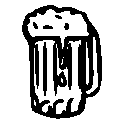
\includegraphics[width=0.5cm]{res/beerpoint.png} }
}

% Die verschiedenen Kategorien für die Punktzahl-Tabelle
\makeatletter
\newcommand{\sauberkeit}{0}
\define@key{fibelbeer}{sauberkeit}{\renewcommand{\sauberkeit}{#1}}
\newcommand{\preisleistung}{0}
\define@key{fibelbeer}{preisleistung}{\renewcommand{\preisleistung}{#1}}
\newcommand{\gemuetlichkeit}{0}
\define@key{fibelbeer}{gemuetlichkeit}{\renewcommand{\gemuetlichkeit}{#1}}
\newcommand{\groesse}{0}
\define@key{fibelbeer}{groesse}{\renewcommand{\groesse}{#1}}
\newcommand{\happyhour}{0}
\define@key{fibelbeer}{happyhour}{\renewcommand{\happyhour}{#1}}
\newcommand{\flirtfaktor}{0}
\define@key{fibelbeer}{flirtfaktor}{\renewcommand{\flirtfaktor}{#1}}
\makeatother

% Befehl "\fibelbeertable": Erstellt eine Tabelle mit den Bierpunkt-Bewertungen
% für eine Disco/Kneipe (inkl. berechneter Gesamtpunktzahl)
%	Parameter: Punktzahlen (0-5) werden in der Form
%	"\fibelbeertable{sauberkeit=<zahl>, ...}" übergeben.
\newcommand{\fibelbeertable}[1]{
\begin{minipage}{\columnwidth}
\setkeys{fibelbeer}{#1}
\centering
\renewcommand{\arraystretch}{1.4}
\begin{tabular}{| l | >{\raggedright\arraybackslash}m{3.65cm} |}
\hline
Sauberkeit		& \fibelbeerscore{\sauberkeit} \\ \hline
Preis/Leistung	& \fibelbeerscore{\preisleistung} \\ \hline
Gemütlichkeit	& \fibelbeerscore{\gemuetlichkeit} \\ \hline
Größe			& \fibelbeerscore{\groesse} \\ \hline
Happy Hour		& \fibelbeerscore{\happyhour} \\ \hline
Flirtfaktor		& \fibelbeerscore{\flirtfaktor} \\ \hline
\end{tabular}\\\medskip

\textbf{Bierpunktzahl insgesamt: \arabic{fibeltotalbeerscore}/30}
\setcounter{fibeltotalbeerscore}{0}
\end{minipage}
}

\section{Der Kneipen-/Disco-Guide für Partypeople!}
\begin{multicols*}{2}
\textbf{Was darf man neben dem Studium auf keinen Fall vergessen? Na, wer weiß es?\\
Richtig, das FEIEEEEERN!!!!!!!!!!!!\\
Damit ihr wisst, wo die Party in Münster geht, stellen wir euch hier den ultimativen Disco- und Kneipenguide vor.}

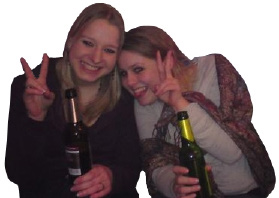
\includegraphics[width=\columnwidth]{res/kneipenguide_foto_silke_annika.png}

Da wir Partylocations bewerten, werden wir ganz stilecht Bierpunkte in den einzelnen Kategorien vergeben. In jeder dieser Kategorien können maximal fünf Bierpunkte erreicht werden. Hier unsere folgenden sechs Bewertungskategorien:

\subsubsection*{Sauberkeit:}
Hier testen wir die Sauberkeit und die Hygiene der Toiletten, sowie die Sauberkeit im Thekenbereich und der gesamten Räumlichkeit.

\subsubsection*{Preis/Leistung:}
Hier testen wir, wie zum Beispiel die Getränkegröße im Verhältnis zum Preis steht, und was man für sein bezahltes Eintrittsgeld geboten bekommt.

\subsubsection*{Gemütlichkeit:}
Hier testen wir die Sitzmöglichkeiten und die Lautstärke der Musik.

\subsubsection*{Größe:}
Hier testen wir, ob die Größe der Räumlichkeiten und der Tanzfläche zum Menschenandrang passend ist.

\subsubsection*{Happy Hours:}
Hier testen wir den zeitlichen Umfang und zudem das Angebot der Happy~Hour.

\subsubsection*{Flirtfaktor:}
Hier Bewerten wir, wie die Singlequote sowie das Flirtverhalten der Partypeople in den jeweiligen Locations ist. Unsere Bewertung bezieht sich auf Erfahrungsberichte diverser Testpersonen ;-)

\subsubsection*{Musik:}
Die Musik wurde von uns nicht bewertet, da die Geschmäcker unterschiedlich sind, jedoch gehen wir in den Texten kurz auf die Auswahl und DJs der einzelnen Clubs ein.

\subsection*{Disco 1: CUBANOVA}
Das Cubanova liegt in der Achtermannstr.~10 direkt am Hbf. In den frühen Abendstunden ist das Cubanova ein Restaurant, wo man für wenig Geld gut essen gehen kann. Nachts, also ab 23:00~Uhr, verwandelt es sich in einen ziemlich geilen Tanzschuppen, mit vielen chilligen Sitzecken. Die Musik ist abwechslungsreich, genau wie die Mottos der Partys, z.B. "Wilde~Hilde" oder die "Disco~2000". Wir raten, erst ab 24:00~Uhr loszuziehen, da vorher dort noch nicht viel los ist. Der Eintritt variiert zwischen \SIrange{3}{5}{\euro}; zusätzlich bezahlt man für die Garderobe \SI{1}{\euro}, diese hat jedoch nicht immer geöffnet.

Niemand hat bis jetzt herausgefunden, nach welchen Kriterien sie öffnen oder schließen. Mittwochs gibt es eine Happy Hour: Sekt/Prosecco/Wein je \SI{1}{\euro}, und von 0:00--1:00~Uhr Flaschenbiere für \SI{1,5}{\euro}.

\begin{center}
\fibelbeertable{sauberkeit=4, preisleistung=2, gemuetlichkeit=5, groesse=3, happyhour=1, flirtfaktor=3}
\end{center}

\subsection*{Disco 2: GOGO}
Das Gogo liegt am Servatiiplatz~1, auch fast direkt am Hbf. Es öffnet seine Türen Mi., Fr. und Sa. ab 22:00~Uhr. Die Musik ist breit gestreut; zu jeder Party kommt das passende, auch wenn es meist eher rocklastig ist. Besonders lohnt es sich, das Gogo mittwochs aufzusuchen, wo eine sehr geile Rockparty läuft. Wer es schafft, vor 23:00~Uhr da zu sein, muss keinen Eintritt zahlen. Danach kostet er \SI{1}{\euro}, genau wie die Garderobe.

Zahlen erledigt man hier nicht direkt, sondern man hat eine Wertkarte, welche das nervige Hantieren mit dem Kleingeld oder Scheinen vermeidet. Jedoch sollte man sie nicht verlieren, denn das wird teuer (\SI{30}{\euro}). Die Happy~Hour des Gogo lautet "Pay~1, Get~2". Diese geht bis 1:00~Uhr, außer Samstags, hier endet sie um 24:00~Uhr. Es gibt eine gemütliche Sitzecke im abgetrennten Raucherbereich.

\begin{center}
\fibelbeertable{sauberkeit=2, preisleistung=5, gemuetlichkeit=3, groesse=4, happyhour=4, flirtfaktor=2}
\end{center}

\subsection*{Disco 3: Eule}
\vspace{-0.3cm}
Die Eule liegt in der Königsstraße~45, also genau in der Innenstadt. In der Eule legt der über die Stadtgrenzen hinweg bekannte DJ~Evo zu den "Fieber-Tanzpartys" auf. Hier läuft moderne Indie-Musik. Am Samstag läuft dann unter dem Motto "Tempocopter" Indierock und Britpop. In der oberen Ebene der Eule ist ein großer Raucherbereich. Unten findet man eine große, rustikal eingerichtete Tanzfläche sowie einen Engtanzraum, in dem konträr zur Rockmusik meistens Elektro läuft. Mit Codewort ist bis 23:30~Uhr der Eintritt kostenlos (Codewort bei Anmeldung für den @-Newsletter). Danach bezahlt man \SIrange{3}{5}{\euro}. Happy~Hour: Beck's und KöPi von 22 bis 0:30~Uhr für \SI{1,50}{\euro} und Pinnchen Mexicana/Sambuca/Tequila die ganze Nacht \SI{1}{\euro}. Die Eule füllt sich jedoch trotz Happy~Hour erst ab 24:00~Uhr.

\begin{center}
\fibelbeertable{sauberkeit=3, preisleistung=4, gemuetlichkeit=5, groesse=3, happyhour=2, flirtfaktor=3}
\end{center}

\subsection*{Disco 4: Schwarzes Schaf}
Das Schwarze~Schaf befindet sich in der Straße Alter~Fischmarkt, also auch noch in der Innenstadt. Es ist in mehrere Räume unterteilt, welche je nach Bedarf und Andrang geöffnet werden. Das Schaf öffnet seine Türen von Mi.--Sa. von 20:00 bis 3:00~Uhr. Im vorderen Bereich hat man das Gefühl, sich in einer hippen Lounge zu befinden. Der Tanzbereich befindet sich im hinteren Teil des Schafs. Die Musik erinnert leicht an Apres~Ski, Fetenhits und Ballermann-Musik. Die Garderobe kostet \SI{2}{\euro}, auch befindet sich ein abgetrennter Raucherbereich im Schaf. Eine Happy~Hour gibt es auch, aber leider nur von 20:00 bis 22:00~Uhr. Hier kostet ein Pils \num{0,3} \SI{1,5}{\euro} und ein Long Island Icetea \SI{3}{\euro}. Jedoch lohnt es sich auch hier trotz der Happy~Hour erst später vorbeizuschauen, denn wirkliche Partystimmung kommt erst später auf.

\begin{center}
\fibelbeertable{sauberkeit=5, preisleistung=3, gemuetlichkeit=2, groesse=4, happyhour=1, flirtfaktor=5}
\end{center}

\subsection*{Kneipe 1: Destille}
Die Destille, auch Dille genannt, befindet sich in der Kuhstraße~10. Diese liegt direkt an der Jüdefelderstraße. Diese wiederum ist bekannt für ihre zahlreichen unterschiedlichen Kneipen. Wir haben uns entschieden, die Dille unter diesem großen Angebot zu testen, da sie eine der bekanntesten und beliebtesten Kneipen der Jüdefelderstraße ist. Das Visage, die Davidswache und die Gorillabar, um nur noch ein paar weitere zu nennen, haben ein ähnliches Konzept.

Die Musik der Destille besteht aus den üblichen Feier- und Partyhits, die jedermann mitsingen kann. Die Happy~Hours bzw. Specials der Dille sind genauso zahlreich wie die Kneipen der Jüdefelderstraße.

Die Destille sollte man relativ früh am Abend aufsuchen, da sie sehr beliebt ist und deshalb einen starken Andrang zu verzeichnen hat. Wer dort zu spät kommt, muss stehen oder bekommt sogar keinen Platz mehr, da die Destille aus einem einzigen Raum besteht. In der Mitte des Raumes befindet sich die Theke; diese ist von allen Seiten aus erreichbar.

Die Destille ist, genau wie die anderen Kneipen der Jüdefelder, der perfekte Ort um sich ohne viel Niveau und günstig zu betrinken bzw. für weitere Aktivitäten vorzuglühen.


\begin{center}
\fibelbeertable{sauberkeit=1, preisleistung=5, gemuetlichkeit=2, groesse=2, happyhour=5, flirtfaktor=4}
\end{center}

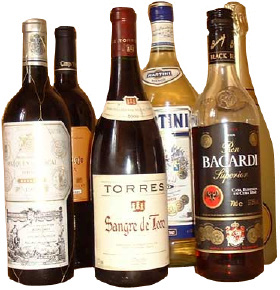
\includegraphics[width=\columnwidth]{res/kneipenguide_flaschen.jpg}

\subsection*{Kneipe 2: Piano}
Das Piano ist eine Karaokebar in der Frauenstraße~46, welche in der Innenstadt liegt. Diese hat Mo.--Do. von 18:00--3:00~Uhr und Fr.--Sa. von 19:00--5:00~Uhr geöffnet.

Die Musik variiert, je nach Wunsch der Gäste, da sie die Stars bzw. Interpreten des Abends sind. Mit einer Auswahl an ungefähr 900~Liedern, die den verschiedensten Musikstilrichtungen entstammen, ist die Musik sehr abwechslungsreich.

Im Piano kann man aber nicht nur singen, sondern auch günstig Alkohol verzehren. Die Happy~Hour, die Mo.--Do. von 18:00--21:00~Uhr, von 1:00--3:00~Uhr und Fr.--Sa. von 19:00--21:00 Uhr, 3:00--4:00~Uhr geht, beinhaltet Hefeweizen für \SI{2,80}{\euro}, Prosecco für \SI{1,50}{\euro} und eine riesige Auswahl an Longdrinks für \SI{1,90}{\euro}.

Das Piano ist eine gemütliche Karaokebar, wo man jede Menge Spaß haben kann mit seinen Freunden und sich nicht nur sinnlos betrinkt. Es ist in zwei Etagen gegliedert, was genügend Sitzmöglichkeiten für alle Gäste ermöglicht. Die Karaokemaschine befindet sich jedoch unten an der Theke in einer Ecke, weshalb man immer seinen Platz verlassen muss, um zu performen. Das Gute daran ist, dass man nicht erst sein Lampenfieber überwinden muss, um auf eine Bühne bzw. Podest zu steigen, da man gemütlich vor der Theke steht, auf gleicher Höhe wie die üblichen Gäste.

\begin{center}
\fibelbeertable{sauberkeit=4, preisleistung=3, gemuetlichkeit=3, groesse=4, happyhour=4, flirtfaktor=1}
\end{center}

\subsection*{Kneipe 3: Himmel und Hölle}
Das Himmel und Hölle liegt in der Kreuzstraße 28/29. Diese Straße ähnelt der Jüdefelder, da sich auch hier eine Menge an Kneipen tummelt, wie z.B. Das~Blaue~Haus oder die Cavete. Die Kreuzstraße befindet sich in der Nähe der Jüdefelder in Richtung Innenstadt.

Diese Kneipe hält Mo.--Sa. von 19:00--3:00~Uhr die Türen für seine Gäste offen. Alternativ, Indie, Rock und Pop sind die Musikrichtungen die dort gespielt werden. Die Happy~Hour gibt es jeden Tag von 20:00--3:00~Uhr. Zu dieser Zeit bestellt man einen Cocktail für \SI{3,90}{\euro}, einen großen Krug gibt es schon für \SI{9,90}{\euro}.

Das Himmel und Hölle betritt man durch einen langen Flur, an dessen Ende man wählen kann, wohin man möchte. Nach links in einen kleinen gemütlichen Raum, oder nach rechts in einen etwas größeren, meist auch volleren Raum, da sich dort die Theke befindet. In den Räumen befinden sich jeweils einige Sitzmöglichkeiten und Stehtische. Während der Happy~Hour ist das Himmel und Hölle meist überfüllt und man steht dicht gedrängt.

\begin{center}
\fibelbeertable{sauberkeit=3, preisleistung=5, gemuetlichkeit=2, groesse=3, happyhour=5, flirtfaktor=2}
\end{center}

\subsection*{Kneipe 4: Gasolin}
In der Nähe des Aasees in der Aegidiistraße~45 befindet sich das Gasolin. Die ehemalige Tankstelle öffnet morgens schon um 11:00~Uhr, da es zu dieser Zeit ein gemütliches und günstiges Café ist (Kaffee: \SI{1,20}{\euro}) und verwandelt sich abends in eine gemütliche Kneipe mit Biergarten (bei gutem Wetter), bis es schließlich um 24:00 Uhr~schließt.

Im Winter bietet das Gasolin den wahrscheinlich günstigsten Glühwein der Stadt an, welcher auch sehr schmackhaft ist. Eine Happy~Hour besitzt das Gasolin zudem auch; mittwochs von 19:00--21:00~Uhr gibt es für ein bezahltes Beck's (\SI{2,30}{\euro}) noch eines geschenkt dazu.

Das Gasolin ist besonders gut geeignet für einen gemütlichen Abend mit Freunden oder ein Abendbier.

\begin{center}
\fibelbeertable{sauberkeit=4, preisleistung=4, gemuetlichkeit=5, groesse=3, happyhour=1, flirtfaktor=1}
\end{center}

\subsection*{Tipps \& Tricks im Nachtleben}
Hier zum Schluss noch ein paar Sachen, die wir euch mit auf den Weg geben wollen.
\begin{itemize}
\item Besucht auf jeden Fall die zahlreichen Parties für Erstsemester, die am Anfang des Semesters angeboten werden. Auch immer wieder zu empfehlen sind die Sportler-Parties.
\item Probiert es aus auch mal, mittwochs feiern zu gehen. Ist zwar am anderen Tag meist Uni, aber es lohnt sich, da sehr viele Studenten an diesem Tag unterwegs sind.
\item Geht am besten nicht zu früh in die Klubs, ab 24:00~Uhr kann man sie gut ansteuern. In die Altstadt kann man an sich nicht zu früh gehen. Ab 21:00~Uhr ist hier am Wochenende oftmals schon was los. Vorher lohnt es sich vorzutrinken, denn auch wenn die Happy~Hours oft gut sind, geht so ein geiler Abend schnell ins Geld.
\item Wenn ihr im Sommer nicht unbedingt Lust habt, in einer stickigen Kneipe zu sitzen, ist es total schön, sich mit ein paar Freunden einen Kasten Bier zu kaufen, und sich gemütlich an den Aasee oder Kanal zu setzen. Ihr werdet feststellen, dass man im Sommer viele Studenten dort trifft, die sich zu einem gemütlichen Bierchen im Freien treffen.
\end{itemize}

\subsection*{Ach ja, noch eine \underline{\smash{Warnung}}!!!}
Sollte es der Fall sein, dass ihr mittwochs feiern gehen wollt, und der darauffolgende Donnerstag ein Feiertag ist, lasst es.

Da Münster sehr viele Gymnasien hat, ist dies ein beliebter Tag für Schüler über 18 Jahren auch mal in der Woche feiern zu gehen, so wie die coolen Studenten. Die Klubs und Bars sind an diesen Tagen mehr als überfüllt!

Sooo, wir hoffen unser Kneipenguide hat euch gefallen und wird euch helfen den Einstieg in Münsters Partyleben leichter zu gestalten, wir hatten auf jeden Fall viel Spaß beim Suchen und Finden der Discos und Kneipen für euch.

\fibelsig{Annika, Silke}
\end{multicols*}
